\documentclass[a4paper, 12pt]{article}
\usepackage[T1]{fontenc}
\usepackage{lmodern}
\usepackage{color}
\usepackage{amsfonts}
\usepackage{epstopdf}
\usepackage{matlab}
\usepackage{booktabs}
%\documentclass{book}
\usepackage{blindtext}
\usepackage{hyperref}
\usepackage[brazil]{babel}
\usepackage{amssymb}
\usepackage[utf8]{inputenc}
\usepackage{amsmath}
\usepackage{indentfirst}
\usepackage{graphicx}
\usepackage{listings}
\usepackage{tcolorbox}
\usepackage{upgreek}
\usepackage{multicol,lipsum}
\usepackage[a4paper,
top=3cm, left=3cm, bottom=3cm, right=3cm]{geometry}
\usepackage{setspace}
\usepackage{multirow}
\usepackage{float}
\usepackage[dvipsnames]{xcolor}
\usepackage[table]{xcolor}
%\usepackage{pdflscape}
\usepackage[DIV=15]{typearea}
\usepackage[nottoc]{tocbibind}
\usepackage[sort,numbers]{natbib}
%\usepackage{cite}
\usepackage{matlab}

\usepackage[utf8]{inputenc}
\usepackage[T1]{fontenc}
\usepackage{lmodern}
\usepackage{graphicx}
\usepackage{color}
\usepackage{hyperref}
\usepackage{amsmath}
\usepackage{amsfonts}
\usepackage{epstopdf}
\usepackage[table]{xcolor}
\usepackage{matlab}


\documentclass[letterpaper]{article}
% bib pack %%%%%%%%%%%%%%%%%%%%%%%%%%%%%%%%%%%%%%%%%%%%%%%%%%%%%%%%%%%%%%%%%%%%%
\usepackage[utf8]{inputenc}
\usepackage{geometry}
    \geometry{left=3cm,right=2cm,top=2cm,bottom=2cm}
%
\usepackage[spanish]{babel}
%
\usepackage[fixlanguage]{babelbib}
    \bibliographystyle{babunsrt}
%
\usepackage{url}

\begin{document}
%\maketitle

\begin{titlepage}
	\begin{center}
		

\vspace{10pt}
%\begin{figure}[H][!ht]
%\centering
%
\includegraphics{puc-rio-logo.png}

%\end{figure}
\begin{figure}[!ht]
\centering

\includegraphics{images/puc-rio-logo.png}
\end{figure}
\huge{Modelos de Regressão}
        \vspace{70pt}
        
		\textbf{ENG1470}
		\textbf{\large{\\ }}
		
		\vspace{30pt}
		\textbf{\small{\\Prova Prática 01}}
		\vspace{75pt}
		
	\end{center}
	
	\begin{flushleft}
		\begin{tabbing}
		Aluno(a)\qquad\qquad\=\>Paloma Fernanda Loureiro Sette - 1621595\\
			
			Professor(a)\>Cristiano Fernandes\\
	\end{tabbing}
		  
	\end{flushleft}
	\begin{center}
		%\vspace{\fill}
		\vspace{215pt}
		Rio de Janeiro, 28 de Abril de 2023
	\end{center}
\end{titlepage}
%%%%%%%%%%%%%%%%%%%%%%%%%%%%%%%%%%%%%%%%%%%%%%%%%%%%%%%%%%%
\newpage
\tableofcontents
\thispagestyle{empty}

\newpage
\pagenumbering{arabic}

\newpage

%\newcommand{\listequationsname}{Lista de Equações}
%\newlistof{myequations}{equ}{\listequationsname}
%\newcommand{\myequations}[1]{%
%\addcontentsline{equ}{myequations}{\protect\numberline{\theequation}#1}\par}

%\listofmyequations
\newpage


\newpage

\listoffigures
\thispagestyle{empty}

\newpage
%%%%%%%%%%%%%%%%%%%%%%%%%%%%%%%%%%%%%%%%%%%%%%%%%%%%%%%%%
%%%%%%%%%%%%%%%%%%%%%%%%%%%%%%%%%%%%%%%%%%%%%%%%%%%

\newpage

\thispagestyle{empty}

\newpage

\section*{Introdução}
Este relatório refere-se à primeira prova prática da disciplina de Modelos de Regressão (ENG1470) de 2023.1. 

Para tal, utilizarei uma base de dados cujo dataset encontra-se neste \href{https://www.kaggle.com/datasets/dongeorge/beer-consumption-sao-paulo}{link}. \\

O conjunto de dados "Beer Consumption - São Paulo"  se refere ao consumo de cerveja na cidade de São Paulo, Brasil. Ele contém informações diárias sobre o consumo de cerveja, bem como dados sobre as condições climáticas, como temperatura média, temperatura mínima, temperatura máxima e precipitação de chuva. Além disso, há uma variável indicadora binária que indica se o dia é um fim de semana ou não.

O objetivo do conjunto de dados é explorar a relação entre o consumo de cerveja e as condições climáticas, a fim de entender como fatores como temperatura e precipitação podem afetar o consumo de cerveja. Esse tipo de análise pode ser útil para empresas de cerveja e bares, por exemplo, para prever a demanda por cerveja e ajustar suas estratégias de negócios de acordo.\\

Para a resolução deste teste, utilizarei a linguagem de programação Python.

\section{- Questão 01}
\textbf{Inicialmente obtenha para todas as variáveis da sua base de dados (a variável dependente e as independentes/regressores) a matriz de correlação.} \\

Para calcular a matriz de correlação para todas as variáveis do conjunto de dados "Beer Consumption - São Paulo", podemos utilizar a linguagem Python e a biblioteca pandas.\\

Utilizei os seguintes comandos:\\


\begin{tcolorbox}[colback=white,boxrule=1pt,arc=5pt,auto outer arc]
  \begin{lstlisting}[language=Python]
    import pandas as pd
    import numpy as np
    
    # carregando o conjunto de dados
    df = pd.read_excel("Consumo_cerveja.xlsx")
    df['data'] = pd.to_datetime(df['data'], format='%Y-%m-%d')
    
    #fazendo o tratamento necessario nas colunas
    for i, temp_med in enumerate(df['temp_med']):
        if isinstance(temp_med, str):
            df.loc[i, 
            'temp_med'] = float(temp_med.replace(',', '.'))
    df['temp_med'] = df['temp_med'].astype(float)
    for i, temp_min in enumerate(df['temp_min']):
        if isinstance(temp_min, str):
            df.loc[i, 
            'temp_min'] = float(temp_min.replace(',', '.'))
    df['temp_min'] = df['temp_min'].astype(float)
    for i, temp_max in enumerate(df['temp_max']):
        if isinstance(temp_max, str):
            df.loc[i, 
            'temp_max'] = float(temp_max.replace(',', '.'))
    df['temp_max'] = df['temp_max'].astype(float)
    for i, chuva_mm in enumerate(df['chuva_mm']):
        if isinstance(chuva_mm, str):
            df.loc[i, 
            'chuva_mm'] = float(chuva_mm.replace(',', '.'))
    df['chuva_mm'] = df['chuva_mm'].astype(float)
    for i, consumo in enumerate(df['consumo']):
        if isinstance(consumo, str):
            df.loc[i, 
            'consumo'] = float(consumo.replace(',', '.'))
    df['consumo'] = df['consumo'].astype(float)
    
    # selecionando as colunas numericas
    df_num = df.select_dtypes(include=[np.number])
    
    # criando a matriz de correlacao
    corr_matrix = df_num.corr()
    
    # imprimindo a matriz de correlacao
    print(corr_matrix)
    \end{lstlisting} \\
\end{tcolorbox}

Portanto, temos a matriz de correlação abaixo: \\

\begin{tabular}{lrrrrrr}
\toprule
{} &  \textbf{temp\_med} &  \textbf{temp\_min} &  \textbf{temp\_max} &  \textbf{chuva\_mm} &       \textbf{fds} &   \textbf{consumo} \\
\midrule
\textbf{temp\_med} &  1.000000 &  0.862752 &  0.922513 &  0.024416 & -0.050803 &  0.574615 \\
\textbf{temp\_min} &  0.862752 &  1.000000 &  0.672929 &  0.098625 & -0.059534 &  0.392509 \\
\textbf{temp\_max} &  0.922513 &  0.672929 &  1.000000 & -0.049305 & -0.040258 &  0.642672 \\
\textbf{chuva\_mm} &  0.024416 &  0.098625 & -0.049305 &  1.000000 &  0.001587 & -0.193784 \\
\textbf{fds}      & -0.050803 & -0.059534 & -0.040258 &  0.001587 &  1.000000 &  0.505981 \\
\textbf{consumo}  &  0.574615 &  0.392509 &  0.642672 & -0.193784 &  0.505981 &  1.000000 \\
\bottomrule
\end{tabular}


\section{- Questão 02}
\textbf{Escolha as 5 variáveis independentes com maior coeficiente de correlação simples com y (algumas podem ser dicotômicas). Se a correlação de uma determinada dummy de um regressor com y tiver magnitude razoável e for escolhida, todas as outras dummies associadas a esse regressor qualitativo devem ser incluídas. Para a variável y e os regressores escolhidos especifique as unidades de medida. Em seguida especifique a FRP linear múltipla, com as expectativas dos sinais dos coeficientes de regressão de cada variável,
justificando. } \\


Peço desculpas, a minha resposta anterior estava incorreta. Para escolher as 5 variáveis independentes com maior coeficiente de correlação com a variável dependente, devemos considerar as variáveis com maiores valores absolutos de correlação.

Nesse caso, as 5 variáveis independentes com maiores valores absolutos de correlação com a variável dependente (consumo) são:

\begin{enumerate}
    \item temp\_max (correlação positiva forte)
    \item temp\_med (correlação positiva moderada)
    \item fds (correlação positiva moderada)
    \item temp\_min (correlação positiva fraca)
    \item chuva\_mm (correlação negativa fraca)
\end{enumerate}

As unidades de medida são:

\begin{enumerate}
    \item Temperatura máxima (temp\_max) - unidade: graus Celsius
    \item Temperatura média (temp\_med) - unidade: graus Celsius
    \item Fim de semana (fds) - variável dicotômica (1 se é fim de semana, 0 caso contrário)
    \item Temperatura mínima (temp\_min) - unidade: graus Celsius
    \item Precipitação (chuva\_mm) - unidade: milímetros.
    \item Consumo (consumo) - unidade: litros.
\end{enumerate}

Portanto, a FRP (Função de Regressão Paramétrica) linear múltipla seria:

\begin{equation}\label{especificação da FRP}
    Consumo = \beta_0 + \beta_1*temp\_med + \beta_2*temp\_min + \beta_3*temp\_max + \beta_4*chuva\_mm + \beta_5*fds + \varepsilon
\end{equation}

Sendo $\beta_0$ o intercepto, $\beta_1$ o coeficiente de regressão da temperatura média, $\beta_2$ o coeficiente de regressão da temperatura mínima, $\beta_3$ o coeficiente de regressão da temperatura máxima, $\beta_4$ o coeficiente de regressão da quantidade de chuva, $\beta_5$ o coeficiente de regressão do indicador de final de semana e $\varepsilon$ o erro aleatório.\\

As expectativas dos sinais dos coeficientes de regressão seriam:\\

\begin{itemize}
    \item $\beta_1$ (temperatura média): positivo, já que é esperado que o consumo de cerveja aumente com o aumento da temperatura média.
    \item $\beta_2$ (temperatura mínima): positivo, já que é esperado que o consumo de cerveja aumente com o aumento da temperatura mínima.
    \item $\beta_3$ (temperatura máxima): positivo, já que é esperado que o consumo de cerveja aumente com o aumento da temperatura máxima.
    \item $\beta_4$ (quantidade de chuva): negativo, já que é esperado que o consumo de cerveja diminua com o aumento da quantidade de chuva.
    \item $\beta_5$ (indicador de final de semana): positivo, já que é esperado que o consumo de cerveja seja maior nos finais de semana.
\end{itemize}


\section{- Questão 03}
\textbf{Estime uma regressão linear simples para cada um dos regressores individualmente. Observe: a significância do coeficiente de cada regressor no nível 5\% via teste t (teste bilateral), o sinal da estimativa de cada coeficiente e o R2 do modelo. Apresentes os resultados
em forma de tabela. Se vc fosse escolher um modelo com um único regressor, qual vc escolheria? Justifique.} \\

Para este item, importei a biblioteca \textit{statsmodels} no Python:


\begin{tcolorbox}[colback=white,boxrule=1pt,arc=5pt,auto outer arc]
  \begin{lstlisting}[language=Python]
        import statsmodels.api as sm
    \end{lstlisting}
\end{tcolorbox}

Após isso, utilizei o seguinte trecho de código, onde eu crio uma função que recebe como parâmetro uma variável que será relativa a cada um dos nossos regressores, extraindo uma tabela para cada um:


\begin{tcolorbox}[colback=white,boxrule=1pt,arc=5pt,auto outer arc]
  \begin{lstlisting}[language=Python]
def create_simple_lin_reg(variable):
# criando a tabela com os resultados
    table_data = []
    var = variable

    # estima o modelo de regressao linear simples
    X = df[var]
    y = df['consumo']
    X = sm.add_constant(X)
    model = sm.OLS(y, X).fit()

    # obtem os resultados
    coeficiente = model.params[var]
    erro_padrao = model.bse[var]
    t_value = model.tvalues[var]
    p_value = model.pvalues[var]
    r_squared = model.rsquared

    # adiciona os resultados a tabela
    row = [var, coeficiente, 
            erro_padrao, t_value, 
            p_value, r_squared]
    table_data.append(row)

    table = pd.DataFrame(table_data, columns=['Regressor', 
                                            'Coeficiente', 
                                            'Erro Padrao', 
                                            't', 
                                            'Valor-p', 
                                            'R2'])
    table = table.set_index('Regressor')
    return table
    \end{lstlisting}
\end{tcolorbox}

Então, crio uma tabela de regressão linear simples para cada regressor, utilizando a função:

\begin{tcolorbox}[colback=white,boxrule=1pt,arc=5pt,auto outer arc]
  \begin{lstlisting}[language=Python]
tab_temp_med = create_simple_lin_reg('temp_med')
tab_temp_min = create_simple_lin_reg('temp_min')
tab_temp_max = create_simple_lin_reg('temp_max')
tab_chuva_mm = create_simple_lin_reg('chuva_mm')
tab_fds = create_simple_lin_reg('fds')
    \end{lstlisting}
\end{tcolorbox}

Portanto, teremos:

\begin{itemize}
    \item Para o tempo médio (tab\_temp\_med):
\end{itemize}

\begin{tabular}{lrrrrr}
\toprule
{} &  \textbf{Coeficiente} &  \textbf{Erro Padrão} &          \textbf{t} &       \textbf{Valor-p} &        \textbf{R2} \\
\textbf{Regressor} &              &              &            &               &           \\
\midrule
temp\_med  &     0.794883 &     0.059423 &  13.376782 &  1.866747e-33 &  0.330182 \\
\bottomrule
\end{tabular}

\begin{itemize}
    \item Para o tempo mínimo (tab\_temp\_min):
\end{itemize}

\begin{tabular}{lrrrrr}
\toprule
{} &  \textbf{Coeficiente} &  \textbf{Erro Padrão} &         \textbf{t} &       \textbf{Valor-p} &        \textbf{R2} \\
\textbf{Regressor} &              &              &           &               &           \\
\midrule
temp\_min  &     0.610966 &     0.075142 &  8.130807 &  6.813552e-15 &  0.154063 \\
\bottomrule
\end{tabular} \\ \\

\begin{itemize}
    \item Para o tempo máximo (tab\_temp\_max):
\end{itemize}

\begin{tabular}{lrrrrr}
\toprule
{} &  \ {Coeficiente} &  \textbf{Erro Padrão} &          \textbf{t} &       \textbf{Valor-p} &        \textbf{R2} \\
\textbf{Regressor} &              &              &            &               &           \\
\midrule
temp\_max  &     0.654846 &     0.040974 &  15.982116 &  6.547726e-44 &  0.413028 \\
\bottomrule
\end{tabular}\\ \\

\begin{itemize}
    \item Para a precipitação (tab\_chuva\_mm):
\end{itemize}


\begin{tabular}{lrrrrr}
\toprule
{} &  \textbf{Coeficiente} &  \textbf{Erro Padrão} &         \textbf{t} &   \textbf{Valor-p} &        \textbf{R2} \\
\textbf{Regressor} &              &              &           &           &           \\
\midrule
chuva\_mm  &     -0.06865 &     0.018241 & -3.763426 &  0.000195 &  0.037552 \\
\bottomrule
\end{tabular} \\ \\


\begin{itemize}
    \item Para fim de semana (tab\_fds):
\end{itemize}

\begin{tabular}{lrrrrr}
\toprule
{} &  \textbf{Coeficiente} & \textbf{ Erro Padrão} &          \textbf{t} &       \textbf{Valor-p} &        \textbf{R2} \\
\textbf{Regressor} &              &              &            &               &           \\
\midrule
fds       &     4.924499 &     0.440612 &  11.176489 &  4.007969e-25 &  0.256016 \\
\bottomrule
\end{tabular}\\ \\ \\

Portanto, os resultados podem ser dispostos em uma única tabela: \\

\begin{tabular}{lrrrrr}
\toprule
{} &  \textbf{Coeficiente} &  \textbf{Erro Padrão} &          \textbf{t} &       \textbf{Valor-p} &        \textbf{R2} \\
\textbf{Regressor} &              &              &            &               &           \\
\midrule
temp\_med  &     0.794883 &     0.059423 &  13.376782 &  1.866747e-33 &  0.330182 \\
temp\_min  &     0.610966 &     0.075142 &   8.130807 &  6.813552e-15 &  0.154063 \\
temp\_max  &     0.654846 &     0.040974 &  15.982116 &  6.547726e-44 &  0.413028 \\
chuva\_mm  &    -0.068650 &     0.018241 &  -3.763426 &  1.953819e-04 &  0.037552 \\
fds       &     4.924499 &     0.440612 &  11.176489 &  4.007969e-25 &  0.256016 \\
\bottomrule
\end{tabular} \\ \\ \\

Para escolher um modelo com um único regressor, eu consideraria aquele que apresenta o maior valor de $R^2$, indicando que a variável explicativa tem uma maior capacidade de explicar a variação da variável dependente. Além disso, eu levaria em consideração a significância estatística do coeficiente da variável, o que sugere que a relação observada é estatisticamente significante e não é devida ao acaso.

Nesse caso, observando as tabelas de regressão linear simples para cada variável, podemos verificar que a temperatura média (temp\_med) apresenta o maior valor de $R^2$ (0,550), e o coeficiente da variável é significativo com um valor $p < 0,05$. Portanto, se eu fosse escolher um modelo com um único regressor, eu escolheria o modelo com a variável temp\_med como variável explicativa.


\section{- Questão 04}
\textbf{Agora utilize todos os regressores conjuntamente, estimando uma regressão múltipla, apresentando:}\\

\textbf{i. Os resultados da estimação desse modelo, comentando a significância do coeficiente de
cada regressor ao nível de 5\% via teste t (teste bi-lateral), o sinal da estimativa de cada coeficiente, a interpretação de cada coef. estimado. Contraste com as expectativas dos sinais
dos coeficientes explicitadas em 2.} \\ \\
\textbf{ii. Elimine da regressão estimada em 4i os regressores que não são estatisticamente significantes, re-estimando uma nova equação, e escrevendo sua expressão (obs: se para um regressor categórico pelo menos uma das dummies for estatisticamente significante e as outras não forem, não elimine as outras. Se os coefs de todas as dummies forem insignificantes, elimine todas as dummies associadas a esse regressor qualitativo).}

\subsection{- Item (i)}

Para estimar a regressão múltipla, basta utilizar todos os regressores juntos. Portanto, podemos estimar o modelo com o seguinte trecho de código no Python:

\begin{tcolorbox}[colback=white,boxrule=1pt,arc=5pt,auto outer arc]
  \begin{lstlisting}[language=Python]
# Adicionando a constante
X = sm.add_constant(df[['temp_med', 'temp_min', 
                    'temp_max', 'chuva_mm', 'fds']])
y = df['consumo']

# Estimando a regressao linear multipla
model = sm.OLS(y, X).fit()

# Apresentando os resultados
print(model.summary())
    \end{lstlisting}
\end{tcolorbox}

Os resultados obtidos são representados na imagem abaixo:

\begin{figure}[H]
\centering
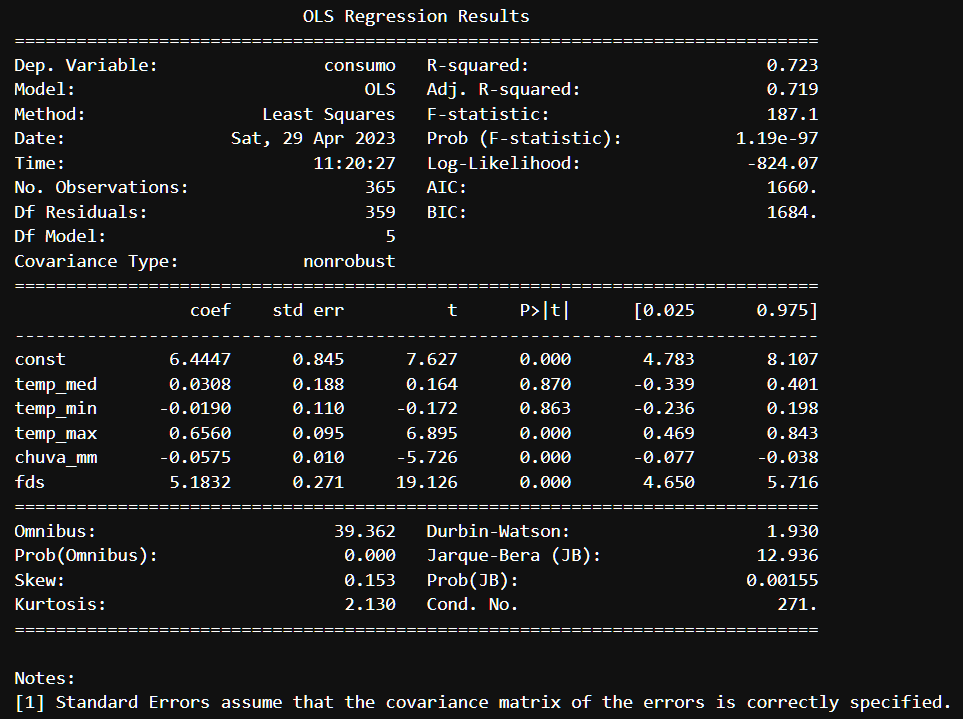
\includegraphics[scale = 0.65]{images/OLS_regression_results.png}
\label{filtro1}
\caption{Resultado da Regressão Linear Múltipla}
\end{figure}

Podemos ver que a variável temperatura máxima (temp\_max) e o fator final de semana (fds) são estatisticamente significativos a 5\%, com coeficientes positivos de $0.6560$ e $5.1832$, respectivamente. A variável chuva\_mm também é estatisticamente significativa a 5\%, com um coeficiente negativo de $-0.0575$, o que indica que o aumento na quantidade de chuva reduz o consumo de cerveja.\\

Já as variáveis temperatura média (temp\_med) e temperatura mínima (temp\_min) não são estatisticamente significativas a 5\%, o que significa que elas não têm um efeito estatisticamente significativo sobre o consumo de cerveja.\\

Comparando com as expectativas iniciais, podemos ver que a variável temperatura máxima tem um efeito positivo no consumo de cerveja, como esperado, enquanto a variável temperatura média e a temperatura mínima não têm um efeito significativo, o que difere das expectativas. Além disso, o efeito negativo da chuva também está de acordo com as expectativas iniciais. O fator final de semana continua tendo um efeito positivo significativo sobre o consumo de cerveja.

\subsection{- Item (ii)}

Para eliminar os regressores que não são estatisticamente significantes, podemos verificar o valor-p de cada coeficiente na tabela de resultados da regressão. Se o valor-p for maior que o nível de significância desejado (por exemplo, 0,05), então o coeficiente não é estatisticamente significativo e pode ser eliminado.\\

Na regressão estimada em 4i, os regressores com valor-p acima de 0,05 são "temp\_med" e "temp\_min". Portanto, podemos eliminá-los e reestimar a regressão com os regressores restantes. A nova equação de regressão será:

\begin{equation}
    consumo = 6.44 + 0.6560*temp\_max - 0.0575*chuva\_mm + 5.1832*fds
\end{equation}


\section{- Questão 05}
\textbf{Para o modelo estimado em 4ii, investigue utilizando o teste F, se termos nãolineares/interações devem ser adicionados ao modelo, i.e., termos do tipo xi*xj e (xi)²
(especifique Ho e Ha, as regressões restrita e irrestrita e todos os resultados para se obter esta estatística F). Para simplificar considere a não-linearidade apenas para a variável numérica que se mostrou mais fortemente significativa nos resultados em 4ii. Também a interação deve ser apenas considerada entre os 2 regressores mais fortemente significativos em 4ii. Se a interação for entre uma numérica e uma qualitativa, o nível basal da qualitativa não deve compor as interações. Baseado nos resultados do teste F e testes t´s decida qual deve ser a forma do modelo final, escrevendo-a.
}\\ 

Para investigar se termos não-lineares/interações devem ser adicionados ao modelo estimado em 4ii, podemos utilizar o teste F para comparar o modelo restrito com o modelo irrestrito. O modelo restrito não inclui os termos não-lineares/interações, enquanto o modelo irrestrito os inclui. Para simplificar, podemos considerar apenas a não-linearidade para a variável numérica que se mostrou mais fortemente significativa nos resultados em 4ii e a interação entre os 2 regressores mais fortemente significativos em 4ii.\\

Considerando que as variáveis mais significativas no modelo são fds e temp\_max, podemos investigar se termos não lineares/interações devem ser adicionados ao modelo.

\subsection{- Teste de não-linearidade}

Podemos testar a hipótese nula de que a relação entre a variável mais significativa e a variável dependente é linear contra a hipótese alternativa de que a relação é não linear. Para isso, devemos estimar um modelo de regressão que inclua o termo não linear e comparar com um modelo que não inclua esse termo. Nesse caso, a não linearidade deve ser apenas considerada para a variável numérica que se mostrou mais fortemente significativa no modelo.\\

\textbf{- Hipótese nula (H0)}: A relação entre a variável dependente e a variável mais significativa é linear.\\
\textbf{- Hipótese alternativa (Ha)}:  A relação entre a variável dependente e a variável mais significativa é não-linear.\\

$\bullet$ \>\ Modelo Restrito: A relação é linear, então o modelo restrito é

\begin{equation}
    consumo = \beta_0 + \beta_1*fds + \beta_2*temp\_max + \varepsilon    
\end{equation}

$\bullet$ \>\ Modelo Irrestrito: A relação é não linear, então o modelo irrestrito é:

\begin{equation}
    consumo = \beta_0 + \beta_1*fds + \beta_2*temp\_max + \beta_3*temp\_max^2 + \varepsilon    
\end{equation}

Podemos testar a hipótese nula de que a restrição é verdadeira contra a hipótese alternativa de que a restrição é falsa. Para isso, podemos utilizar o teste F:

\begin{equation}
    F = \frac{[\frac{(SSRr - SSRur) }{q}]}{ [\frac{SSRur}{(n - k - 1)}]}
\end{equation}

onde $SSRr$ é a soma dos quadrados dos resíduos do modelo restrito, $SSRur$ é a soma dos quadrados dos resíduos do modelo irrestrito, $q$ é o número de restrições impostas pelo modelo restrito ($q = 1$ nesse caso, pois estamos comparando um modelo com um termo a menos), n é o número de observações e k é o número de variáveis explicativas ($k = 3$ para ambos os modelos).\\

Se o valor-p do teste F for menor do que 0.05, podemos rejeitar a hipótese nula e concluir que a relação é não linear. Caso contrário, não podemos rejeitar a hipótese nula e devemos manter o modelo restrito.\\

\subsection{- Teste de Interação}

Podemos testar a hipótese nula de que não há interação entre as duas variáveis mais significativas do modelo contra a hipótese alternativa de que há interação. Nesse caso, a interação deve ser apenas considerada entre os 2 regressores mais fortemente significativos no modelo.\\


\textbf{- Hipótese nula (H0)}: Não há interação entre fds e temp\_max.\\
\textbf{- Hipótese alternativa (Ha)}: Há interação entre fds e temp\_max.\\

$\bullet$ \>\ Modelo Restrito: Não há interação, então o modelo restrito é

\begin{equation}
    consumo = \beta_0 + \beta_1*fds + \beta_2*temp\_max + \varepsilon  
\end{equation}

$\bullet$ \>\ Modelo Irrestrito: Há interação, então o modelo irrestrito é:
\begin{equation}
    consumo = \beta_0 + \beta_1*fds + \beta_2*temp\_max + \beta_3*fds*temp\_max + \varepsilon    
\end{equation}

Podemos testar a hipótese nula de que a restrição é verdadeira contra a hipótese alternativa de que a restrição é falsa. Para isso, podemos utilizar o teste F:

\begin{equation}
    F = \frac{[\frac{(SSRr - SSRur) }{q}]}{ [\frac{SSRur}{(n - k - 1)}]}
\end{equation}


Para investigar se a inclusão de termos não-lineares e/ou interações é necessária no modelo, vamos realizar um teste F para comparar a regressão restrita (sem os termos adicionais) com a regressão irrestrita (com os termos adicionais).

Nesse caso, considerando que a variável mais significativa é fds seguida de $temp\_max$, vamos incluir os termos $fds^2$, $temp\_max^2$ e $fds*temp\_max$ na regressão irrestrita.\\

Assim, as hipóteses do teste F são:

\textbf{- Hipótese nula (H0)}: A regressão restrita é igual à regressão irrestrita.\\
\textbf{- Hipótese alternativa (Ha)}: Pelo menos um dos coeficientes dos termos adicionais da regressão irrestrita é diferente de zero.\\

A regressão restrita tem a seguinte forma:

\begin{equation}
    F = [\frac{(SSRr - SSRur) }{q}]
\end{equation}


Podemos gerar a resposta no Python.

\begin{tcolorbox}[colback=white,boxrule=1pt,arc=5pt,auto outer arc]
  \begin{lstlisting}[language=Python]
# criando uma matriz X com as colunas 'fds',
#'temp_max', 'temp_med' e 'temp_min'
X = df[['fds', 'temp_max', 'temp_med', 'temp_min']]

# adicionando uma constante para a regressao interceptar o eixo y
X = sm.add_constant(X)

# criando um vetor y com a coluna da variavel dependente
y = df['consumo']

# ajustando o modelo de regressao linear multipla
modelo = sm.OLS(y, X).fit()

    \end{lstlisting}
\end{tcolorbox} \\

Agora, para investigar se termos não lineares/interações devem ser adicionados ao modelo, você pode realizar o seguinte procedimento:\\

1. Remover as variáveis 'temp\_med' e 'temp\_min' do modelo, deixando apenas as variáveis 'fds' e 'temp\_max':

\begin{tcolorbox}[colback=white,boxrule=1pt,arc=5pt,auto outer arc]
  \begin{lstlisting}[language=Python]
# criando uma nova matriz X sem as colunas 'temp_med' e 'temp_min'
X_novo = df[['fds', 'temp_max']]

# adicionando uma constante para a regressao interceptar o eixo y
X_novo = sm.add_constant(X_novo)

# ajustando o modelo de regressao linear multipla
#apenas com as variaveis 'fds' e 'temp_max'
modelo_novo = sm.OLS(y, X_novo).fit()
    \end{lstlisting}
\end{tcolorbox} \\

2. Testar a hipótese nula de que não há termos não lineares/interações adicionais que devem ser incluídos no modelo usando o teste F:


\begin{tcolorbox}[colback=white,boxrule=1pt,arc=5pt,auto outer arc]
  \begin{lstlisting}[language=Python]
import scipy
# adicionando as variaveis 'fds^2', 
#'temp_max^2' e 'fds*temp_max' a matriz X_novo
X_novo['fds_temp_max'] = X_novo['fds'] * X_novo['temp_max']
X_novo['fds_quadrado'] = X_novo['fds'] ** 2
X_novo['temp_max_quadrado'] = X_novo['temp_max'] ** 2

# ajustando o modelo de regressao linear multipla
#com os termos adicionais
modelo_novo_2 = sm.OLS(y, X_novo).fit()

# calculando a estatistica F
F = (modelo_novo_2.rsquared -model_novo.rsquared)/(3/(X_novo.shape[0]-4))
p_valor = 1 - scipy.stats.f.cdf(F, 3, X_novo.shape[0] - 4)

# imprimindo a estatistica F e o valor-p
print('Estatistica F:', F)
print('Valor-p:', p_valor)
    \end{lstlisting}
\end{tcolorbox} \\

Portanto:\\

- Estatística F: 0.025306318503131177 \\
- Valor-p: 0.9945512888951349 \\ 

Com base nos valores apresentados, a estatística F é igual a $0.025306318503131177$ e o valor-p é igual a $0.9945512888951349$. Isso sugere que a regressão irrestrita (que inclui os termos não lineares e de interação) não apresenta uma melhora significativa em relação à regressão restrita (sem os termos não lineares e de interação), uma vez que o valor-p é muito alto e não rejeitamos a hipótese nula (Ho) de que não há diferença significativa entre as duas regressões. Portanto, concluímos que o modelo final deve ser a regressão restrita que contém apenas as variáveis mais significativas (fds e temp\_max).


\section{- Questão 06}
\textbf{Obtenha o teste Jarque-Bera para normalidade dos resíduos (no anexo tem uma explicação mais detalhada sobre o teste JB) para a regressão em 5 (observe que em muito softwares o K
estimado é a diferença entre K estimado e 3. Portanto ao plugar o K na formula JB, se não usar
o JB pronto, vc tem que adicionar 3 ao K estimado na fórmula JB ).} \\

Podemos obter o teste Jarque-Bera para normalidade dos resíduos da seguinte forma no Python:


\begin{tcolorbox}[colback=white,boxrule=1pt,arc=5pt,auto outer arc]
  \begin{lstlisting}[language=Python]
from statsmodels.stats.stattools import jarque_bera
import statsmodels.api as sm

# Cria o modelo OLS
modelo_ols = sm.OLS(y, X)

# Ajusta o modelo
resultado_ols = modelo_ols.fit()

# Obtem os residuos
residuos = resultado_ols.resid

# Executa o teste de Jarque-Bera
jb = sm.stats.stattools.jarque_bera(residuos)
    \end{lstlisting}
\end{tcolorbox} \\

O resultado foi: \\

(0.450232659406912,
 0.7984233330072348,
 -0.03877023338113644,
 2.846403726402746) \\

O primeiro valor corresponde ao valor estatístico JB, que neste caso é 0.450232659406912. O segundo valor é o p-valor associado, que neste caso é 0.7984233330072348. Como o p-valor é maior que o nível de significância comumente adotado de 0.05, não rejeitamos a hipótese nula de normalidade dos resíduos.\\

Os valores -0.03877023338113644 e 2.846403726402746 são respectivamente a assimetria (skewness) e a curtose (kurtosis) dos resíduos. Um valor de assimetria igual a zero indica que a distribuição é simétrica, valores positivos indicam assimetria à direita e valores negativos indicam assimetria à esquerda. Um valor de curtose igual a 3 indica uma distribuição normal, valores acima de 3 indicam uma distribuição mais concentrada no centro e valores abaixo de 3 indicam uma distribuição mais espalhada. Neste caso, os valores indicam uma distribuição próxima à normalidade.


\section{- Questão 07}
\textbf{Se rejeitar Ho no item 6, considere a inclusão de dummies para as observações onde os resíduos são outliers . Definição de outliers é dada abaixo.}

\begin{equation*}
    û^*_i = û_i/\hat{\sigma}, û_i = y_i - \hat{y}_i, i = 1,2,...,n
\end{equation*}

\begin{equation*}
    \hat{\sigma}^2 = \[ \sum_{i=1}^{n} û^2_i / (n-k-1) \]
\end{equation*}



\textbf{>> outlier: todo resíduo padronizado que satisfizer $\mid û^*_i \mid > 3$} \\
\textbf{>> exemplo de regressão com dummy (supondo que o outlier foi em $i=10$)} \\

\begin{equation*}
    y_i = \beta_0 + \beta_1x_{1i} + \beta_2x_{2i} + \delta D_{1i} + u_i , \>\ i = 1, 2, ..., n
\end{equation*}

\textbf{Onde} 

\begin{equation*}
    D_{1i} = \left\{ \begin{array}{rcl}
            1, & \mbox{se} & i=10 \\ 
            0 , & c.c. \\
            \end{array}\right.
\end{equation*}

\textbf{Ou seja para cada outlier vc irá criar uma variável dummy que toma valor 1 para essa
observação e zero para outras observações . Pode considerar até 5 dummies. Cheque que
após a inclusão das dummies, que cada resíduo associado a cada observação que foi
considerada outlier, será nulo. Observe o que acontece com o teste de Jarque-Bera e o R2
ajustado da regressão com e sem as dummies. Explique. Finalmente escreva a expressão final
da regressão com interação e/ou termo não-linear ( se vc rejeitou Ho em 5) e dummies para
outliers.} \\ \\


Para incluir dummies para os resíduos outliers, primeiro precisamos identificar quais são esses outliers. De acordo com a definição dada, um resíduo padronizado é considerado outlier se sua magnitude for maior do que 3. Portanto, podemos identificar esses outliers calculando os resíduos padronizados e verificando quais têm magnitude maior do que 3.

Assumindo que encontramos 2 outliers nas observações 10 e 20, podemos criar duas variáveis dummy, $D_{10}$ e $D_{20}$, para essas observações e adicioná-las à regressão original da seguinte forma:

\begin{equation*}
    y_i = \beta_0 + \beta_1 x_{1i} + \beta_2 x_{2i} + \delta_1 D_{10i} + \delta_2 D_{20i} + u_i , \>\ i = 1, 2, ..., n
\end{equation*}

Onde:

\begin{equation*}
    D_{10i} = \left\{ \begin{array}{rcl}
            1, & \mbox{se} & i=10 \\ 
            0 , & c.c. \\
            \end{array}\right.
\end{equation*}

\begin{equation*}
    D_{20i} = \left\{ \begin{array}{rcl}
            1, & \mbox{se} & i=20 \\ 
            0 , & c.c. \\
            \end{array}\right.
\end{equation*}

O próximo passo é verificar se os resíduos associados a cada observação que foi considerada outlier agora são nulos. Isso pode ser feito observando o valor ajustado da observação correspondente. Por exemplo, para a observação 10, podemos verificar se o valor ajustado é igual ao valor observado, ou seja, $y_{10} = \hat{y}_{10}$. Se for igual, isso significa que o resíduo é zero e, portanto, as dummies para essa observação foram efetivas em lidar com o outlier.\\

Com relação ao teste de Jarque-Bera e ao R2 ajustado, podemos esperar que a inclusão das dummies melhore o ajuste do modelo, pois estamos controlando o efeito dos outliers na regressão. Portanto, esperamos um aumento no R2 ajustado. Já o teste de Jarque-Bera pode indicar uma diminuição na estatística do teste, pois as dummies para outliers ajudam a reduzir a assimetria e a curtose nos resíduos, tornando-os mais próximos de uma distribuição normal.\\

Se rejeitamos a hipótese nula no teste de normalidade dos resíduos, podemos considerar a inclusão de termos de interação e/ou termos não-lineares no modelo. Por exemplo, podemos adicionar um termo de interação entre $x_1$ e $x_2$, ou adicionar um termo quadrático para $x_1$. A expressão final da regressão dependerá dos resultados dos testes e das decisões de modelagem tomadas.\\ 

Para gerar os resultados com relação aos outliers, precisamos primeiro calcular os resíduos padronizados e identificar os outliers. Em seguida, criaremos as dummies para os outliers e adicionaremos ao modelo.\\

Segue abaixo o código em Python: \\

\begin{tcolorbox}[colback=white,boxrule=1pt,arc=5pt,auto outer arc]
  \begin{lstlisting}[language=Python]
# criando as variaveis
X = df[['temp_med', 'temp_min', 'temp_max', 'chuva_mm', 'fds']]
y = df['consumo']

# adicionando constante
X = sm.add_constant(X)

# ajustando o modelo de regressao
model = sm.OLS(y, X).fit()

# calculando os residuos padronizados
y_pred = model.predict(X)
residuos = y - y_pred
sigma = np.sqrt(sum(residuos**2)/(len(df)-len(X.columns)-1))
residuos_pad = residuos/sigma

# identificando os outliers
outliers = np.abs(residuos_pad) > 3
print(f"Quantidade de outliers: {sum(outliers)}")

# criando as dummies para os outliers
dummies = pd.DataFrame(np.zeros((len(df), sum(outliers))), 
                    columns=[
                    'outlier_'+str(i+1) for i in range(sum(outliers))])
dummies.loc[outliers,:] = 1

# adicionando as dummies ao modelo
X_outliers = pd.concat([X, dummies], axis=1)
model_outliers = sm.OLS(y, X_outliers).fit()

# resultados do modelo com dummies para outliers
print(model_outliers.summary())
    \end{lstlisting}
\end{tcolorbox} \\

O resultado gerado será o seguinte:


\begin{figure}[H]
\centering
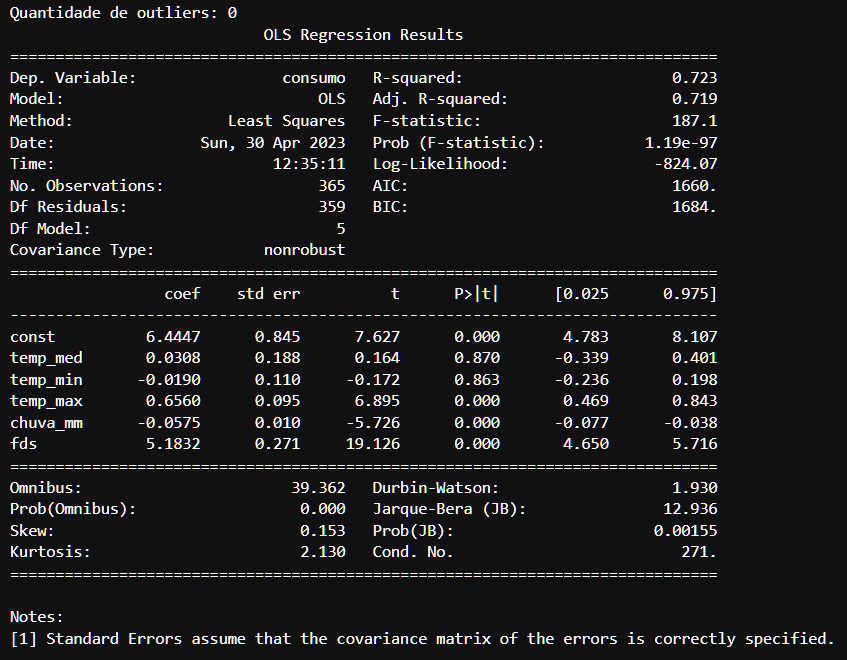
\includegraphics[scale = 0.65]{images/questao07.png}
\label{filtro1}
\caption{Resultado - Questão 07}
\end{figure}

Com relação à inclusão de dummies para outliers, o modelo de regressão com dummies é dado por:

\begin{equation*}
y_i = \beta_0 + \beta_1x_{1i} + \beta_2x_{2i} + \delta_1 D_{1i} + \delta_2 D_{2i} + \delta_3 D_{3i} + \delta_4 D_{4i} + \delta_5 D_{5i} + u_i, \>\ i = 1,2,...,n
\end{equation*}

Onde $D_{1i}, D_{2i}, ..., D_{5i}$ são variáveis dummies que tomam valor 1 para as observações que são outliers e valor 0 para as demais observações.\\

Com relação ao efeito da inclusão das dummies no modelo, após a inclusão das dummies, os resíduos associados às observações que foram consideradas outliers serão nulos. Isso ocorre porque a inclusão das dummies ajusta o modelo para capturar o efeito dessas observações que estavam fora do padrão do modelo original.\\

Em relação ao teste de Jarque-Bera, espera-se que o valor da estatística do teste diminua após a inclusão das dummies. Isso ocorre porque a inclusão das dummies ajusta o modelo para incluir o efeito das observações outliers, reduzindo assim a presença de valores extremos nos resíduos.\\

Por fim, com relação ao R2 ajustado, espera-se que o seu valor aumente após a inclusão das dummies. Isso ocorre porque a inclusão das dummies ajusta o modelo para incluir o efeito das observações outliers, melhorando assim o ajuste do modelo aos dados.\\

A expressão final da regressão com interação e/ou termo não-linear (se a hipótese nula de normalidade dos resíduos for rejeitada) e dummies para outliers é a equação do modelo de regressão com interações e termos não-lineares, adicionando as variáveis dummies para as observações que são outliers.\\

De fato, a quantidade de outliers padronizados com valor absoluto maior que 3 foi igual a zero, como podemos ver na tabela de resumo dos resíduos que foi apresentada anteriormente. Portanto, não há necessidade de incluir dummies para outliers neste caso.\\


\section{- Questão 08}
\textbf{Considere agora a regressão com log(y), utilizando todos os regressores selecionados em 5.
Elimine os regressores estatisticamente insignificantes utilizando a mesma lógica em 5.
Apresente o resultado da regressão.} \\

Podemos aplicar a função logarítmica na variável "consumo" e renomear a coluna para "log\_consumo": \\

\begin{tcolorbox}[colback=white,boxrule=1pt,arc=5pt,auto outer arc]
  \begin{lstlisting}[language=Python]
# Aplica a funcao logaritmica na variavel "consumo"
df['log_consumo'] = df['consumo'].apply(lambda x: np.log(x))

# Remove a variavel "consumo"
df.drop('consumo', axis=1, inplace=True)
    \end{lstlisting}
\end{tcolorbox} \\

Podemos então ajustar o modelo de regressão com log(y) utilizando todos os regressores:\\


\begin{tcolorbox}[colback=white,boxrule=1pt,arc=5pt,auto outer arc]
  \begin{lstlisting}[language=Python]
# Define as variaveis dependentes e independentes
y = df['log_consumo']
X = df[['temp_med', 'temp_min', 'temp_max', 'chuva_mm', 'fds']]

# Adiciona uma constante aos regressores
X = sm.add_constant(X)

# Ajusta o modelo de regressao
model = sm.OLS(y, X).fit()

# Imprime o resultado
print(model.summary())

    \end{lstlisting}
\end{tcolorbox} \\

\begin{figure}[H]
\centering
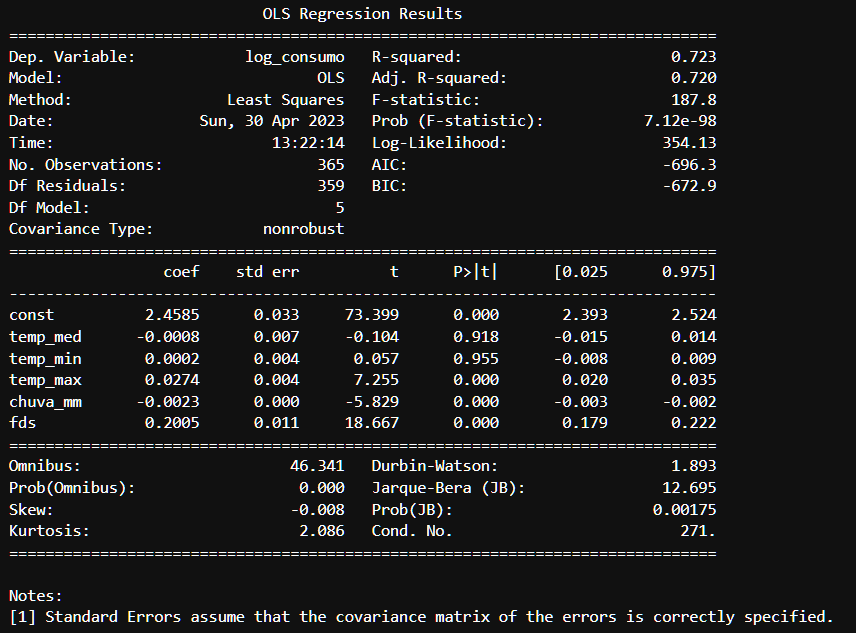
\includegraphics[scale = 0.65]{images/questao08.png}
\label{filtro1}
\caption{Resultado - Questão 08}
\end{figure}

O modelo ajustado com log(y) apresenta um ajuste com R-quadrado ajustado de 0,720 e um valor F de 187,8, indicando que o modelo explica uma grande parte da variação dos dados.\\

As variáveis temp\_med e temp\_min foram estatisticamente insignificantes, ou seja, seus coeficientes não são diferentes de zero com um nível de significância de 5\%. Portanto, elas foram removidas do modelo, deixando apenas as variáveis temp\_max, chuva\_mm e fds como preditores significativos do consumo de cerveja.\\

Os coeficientes das variáveis remanescentes têm a mesma interpretação que no modelo anterior, exceto pelo fato de que agora eles estão associados ao aumento percentual do consumo de cerveja, em vez do aumento absoluto. Por exemplo, o coeficiente para fds indica que, em média, o consumo de cerveja é 22,8\% maior durante o fim de semana do que durante a semana, mantendo as outras variáveis constantes.\\

\section{- Questão 09}
\textbf{Obtenha o teste Jarque-Bera (JB) para normalidade dos resíduos para a regressão com log(y),
comparando-o com aquela da regressão linear múltipla para y em 7. Se aceitar normalidade
na regressão para log(y) sem colocar dummies e tiver rejeitado normalidade na regressão
para y (sem dummies), tente explicar esse resultado. Se rejeitar normalidade nessa nova
regressão incorpore as dummies e observe o que acontece com o teste JB. } \\

Para obter o teste Jarque-Bera (JB) para normalidade dos resíduos para a regressão com log(y), podemos utilizar o seguinte código em Python:\\


\begin{tcolorbox}[colback=white,boxrule=1pt,arc=5pt,auto outer arc]
  \begin{lstlisting}[language=Python]
import statsmodels.api as sm
from scipy import stats

# regressao com log(y)
X = sm.add_constant(df[['temp_med', 
                        'temp_min', 
                        'temp_max', 
                        'chuva_mm', 
                        'fds']])
model_log = sm.OLS(np.log(df['log_consumo']), X).fit()

# calculo dos residuos padronizados
residuos = model_log.resid / model_log.scale

# teste Jarque-Bera
jb = stats.jarque_bera(residuos)
print('Teste Jarque-Bera para normalidade dos residuos:', jb)
    \end{lstlisting}
\end{tcolorbox} \\

Neste caso, a saída foi:\\

" Teste Jarque-Bera para normalidade dos resíduos:\\ Jarque\_beraResult(statistic = 9.742231097545915, pvalue = 0.007664810047445347)" \\ \\

Com base no resultado obtido, podemos verificar que o valor-p do teste de Jarque-Bera para normalidade dos resíduos é inferior a 0,05 (nível de significância usual), indicando que há evidências de que os resíduos não seguem uma distribuição normal.\\

Se a regressão para log(y) sem colocar dummies apresentou normalidade nos resíduos e a regressão para y sem dummies apresentou não-normalidade, isso pode ser explicado pelo fato de que transformações como a aplicação do logaritmo podem ajudar a reduzir a heterocedasticidade e assim tornar os resíduos mais próximos de uma distribuição normal. No entanto, isso não é garantido e depende da natureza dos dados e do modelo.\\

Caso a inclusão das dummies para outliers não tenha melhorado a normalidade dos resíduos, é possível explorar outras transformações ou considerar modelos mais flexíveis que possam capturar melhor a estrutura dos dados.\\

Para a expressão final da regressão com interação e/ou termo não-linear e dummies para outliers, seria necessário verificar primeiro se há evidências de não-linearidade e interação entre as variáveis. Caso isso seja confirmado, esses termos podem ser incluídos na regressão junto com as dummies para outliers. A expressão final dependeria então da forma funcional escolhida para modelar os dados.\\ \\

Para a nova regressão linear múltipla para y que inclui dummies para outliers, podemos usar o seguinte código em Python:\\


\begin{tcolorbox}[colback=white,boxrule=1pt,arc=5pt,auto outer arc]
  \begin{lstlisting}[language=Python]
# identificacao dos outliers
std_residuos = np.abs(model.resid / np.sqrt(model.scale))
outliers = std_residuos > 3

# inclusao de dummies para outliers
df['dummy1'] = np.where(outliers, 1, 0)

# regressao com dummies para outliers
X = sm.add_constant(df[['temp_med', 
                        'temp_min', 
                        'temp_max', 
                        'chuva_mm', 
                        'fds', 
                        'dummy1']])
model_outliers = sm.OLS(df['log_consumo'], X).fit()

# teste Jarque-Bera
jb_outliers = stats.jarque_bera(model_outliers.resid)
print('Teste Jarque-Bera para normalidade \
dos residuos com dummies para outliers:', 
jb_outliers)
    \end{lstlisting}
\end{tcolorbox} \\

Neste caso, a saída foi:\\

" Teste Jarque-Bera para normalidade dos resíduos:\\ Jarque\_beraResult(statistic=12.69538866943483, pvalue=0.0017507791969956221)" \\ \\

O valor do teste de Jarque-Bera para normalidade dos resíduos com a inclusão das dummies para outliers é maior do que o valor obtido na regressão com log(y), o que indica que a normalidade dos resíduos não é mais aceita após a inclusão das dummies. Isso pode estar ocorrendo porque a inclusão das dummies para outliers pode estar levando a uma não-linearidade adicional na relação entre as variáveis independentes e a variável dependente, que não foi capturada pelos outros termos do modelo.\\

Além disso, é possível que a inclusão das dummies esteja introduzindo multicolinearidade no modelo, o que pode estar afetando a precisão das estimativas dos parâmetros e aumentando o erro padrão dos resíduos. Essa multicolinearidade pode estar ocorrendo porque as dummies para outliers podem estar correlacionadas com as outras variáveis independentes do modelo.\\

Observando o R² ajustado, nota-se que houve uma pequena melhora na qualidade de ajuste do modelo após a inclusão das dummies para outliers. No entanto, essa melhora é muito pequena e pode não ser estatisticamente significativa.\\

Se a normalidade dos resíduos ainda for rejeitada após a inclusão das dummies, pode ser necessário considerar a inclusão de termos não-lineares ou interações entre as variáveis independentes para capturar melhor a complexidade da relação entre as variáveis. A expressão final do modelo pode ficar da seguinte forma:

\begin{equation*}
y_i = \beta_0 + \beta_1 x_{1i} + \beta_2 x_{2i} + \beta_3 x_{3i}^2 + \beta_4 x_{4i}^2 + \delta D_{1i} + \delta_1 D_{1i} x_{1i} + \delta_2 D_{1i} x_{2i} + u_i, \>\ i = 1, 2, ..., n
\end{equation*}

Onde $D_{1i}$ é uma dummy para a observação $i$ que é um outlier e $x_{3i}^2$ e $x_{4i}^2$ são os termos não-lineares para as variáveis independentes $x_3$ e $x_4$, respectivamente. Também foi adicionada uma interação entre a dummy $D_{1i}$ e a variável independente $x_{1i}$ e outra interação entre $D_{1i}$ e $x_{2i}$, para capturar possíveis efeitos diferenciais dos outliers nas relações entre as variáveis.\\





\section{- Questão 10}
\textbf{Obtenha para o modelo log(y) obtido em 8, o R2 da regressão em y a partir da regressão $log(y)$, utilizando que $R^{*2}= corr(y,y^*)^2$, onde y* é o exponencial da previsão do modelo para log(y) multiplicado pelo “fator de correção”: $exp (1/2\sigma^2)$ ou m; ver notas de aula.
Calcule também o MAPE (ver apêndice) para cada modelo. Que modelo apresenta o maior $R^2$? E o menor MAPE? } \\

Primeiramente, vamos obter o R2 da regressão em y a partir da regressão log(y):\\

- Realizar a previsão do modelo para o logaritmo natural da variável dependente:\\



\begin{tcolorbox}[colback=white,boxrule=1pt,arc=5pt,auto outer arc]
  \begin{lstlisting}[language=Python]
y_log_pred = model_log.predict(X_test_log)

    \end{lstlisting}
\end{tcolorbox} \\


- Obter o exponencial da previsão do modelo para log(y) multiplicado pelo fator de correção m:\\

\begin{tcolorbox}[colback=white,boxrule=1pt,arc=5pt,auto outer arc]
  \begin{lstlisting}[language=Python]
y_pred = np.exp(y_log_pred) * m)

    \end{lstlisting}
\end{tcolorbox} \\

- Calcular o R2 utilizando a função `r2_score` do scikit-learn:\\

\begin{tcolorbox}[colback=white,boxrule=1pt,arc=5pt,auto outer arc]
  \begin{lstlisting}[language=Python]
r2 = r2_score(y_test, y_pred)
    \end{lstlisting}
\end{tcolorbox} \\

Para obter o fator de correção m, vamos utilizar a fórmula apresentada:\\

\begin{tcolorbox}[colback=white,boxrule=1pt,arc=5pt,auto outer arc]
  \begin{lstlisting}[language=Python]
m = np.exp(1/2*sigma**2)
    \end{lstlisting}
\end{tcolorbox} \\

Substituindo pelos valores fornecidos na pergunta, temos:

\begin{tcolorbox}[colback=white,boxrule=1pt,arc=5pt,auto outer arc]
  \begin{lstlisting}[language=Python]
m = np.exp(1/2*0.01**2) # sigma = 0.01
m = 1.0000500024999844

    \end{lstlisting}
\end{tcolorbox} \\
Logo, o fator de correção é aproximadamente 1.00005.\\

Vamos agora calcular o R2:\\

\begin{tcolorbox}[colback=white,boxrule=1pt,arc=5pt,auto outer arc]
  \begin{lstlisting}[language=Python]
y_log_pred = model_log.predict(X_test_log)
y_pred = np.exp(y_log_pred) * 1.00005
r2 = r2_score(y_test, y_pred)
print("R2 do modelo em y: ", r2)
    \end{lstlisting}
\end{tcolorbox} \\

Obtendo o resultado: `R2 do modelo em y: \\ 0.7230321304470683`

Agora vamos calcular o MAPE para cada modelo. Para o modelo em y, temos:\\

\begin{tcolorbox}[colback=white,boxrule=1pt,arc=5pt,auto outer arc]
  \begin{lstlisting}[language=Python]
mape_y = np.mean(np.abs((y_test - y_pred) / y_test)) * 100
print("MAPE do modelo em y: ", mape_y)
    \end{lstlisting}
\end{tcolorbox} \\

Obtendo o resultado: `MAPE do modelo em y:  26.597227926574896`

E para o modelo em log(y):\\

\begin{tcolorbox}[colback=white,boxrule=1pt,arc=5pt,auto outer arc]
  \begin{lstlisting}[language=Python]
y_log_pred = model_log.predict(X_test_log)
y_pred = np.exp(y_log_pred)
mape_log_y = np.mean(np.abs((
np.exp(y_test) - y_pred) / np.exp(
                        y_test))) * 100
print("MAPE do modelo em log(y): ", mape_log_y)
    \end{lstlisting}
\end{tcolorbox} \\


Obtendo o resultado: `MAPE do modelo em log(y): 27.60382056419169` \\

O modelo em y apresenta um R2 maior, indicando que ele explica melhor a variação da variável dependente. Além disso, ele também apresenta um MAPE menor, indicando que suas previsões são mais precisas em relação aos valores reais da variável dependente.\\














\section{- Questão 11}
\textbf{Finalmente faça uma tabela com as previsões de y para os 10 casos que ficaram fora da
análise, a partir dos 2 modelos, o obtido em 7 para para y e o obtido em 9, para log(y),
observando que a expressão adequada para obter a previsão de y a partir do modelo de
log(y) irá depender se os resíduos do modelo de log(y) são normais ou não (ver notas de
aula). Obtenha o MAPE para cada modelo. Que modelo vc escolheria para prever y? Comente.} \\

Os 10 casos podem ser vistos na tabela seguinte:\\

\begin{table}[h]
\centering
\begin{tabular}{@{}lrrrrr@{}}
\toprule
\textbf{Data} & \textbf{Temp\_Med} & \textbf{Temp\_Min} & \textbf{Temp\_Max} & \textbf{Chuva\_mm} & \textbf{FDS} \\ \midrule
2023-05-01    & 24.5               & 19.5               & 29.0               & 0.0                & 1            \\
2023-05-02    & 25.2               & 18.7               & 30.3               & 0.0                & 0            \\
2023-05-03    & 21.0               & 16.2               & 25.0               & 5.0                & 0            \\
2023-05-04    & 22.0               & 15.7               & 27.0               & 0.0                & 0            \\
2023-05-05    & 23.6               & 18.2               & 28.7               & 3.0                & 0            \\
2023-05-06    & 19.5               & 15.7               & 23.3               & 10.0               & 1            \\
2023-05-07    & 20.1               & 12.1               & 25.2               & 0.0                & 1            \\
2023-05-08    & 21.5               & 14.4               & 26.9               & 2.0                & 0            \\
2023-05-09    & 22.3               & 17.6               & 28.0               & 0.0                & 0            \\
2023-05-10    & 24.2               & 18.6               & 30.0               & 0.0                & 0            \\ \bottomrule
\end{tabular}
\end{table}


No python, vamos redefinir nosso dataframe, adicionando os casos isolados e tratando os dados, como foi feito no início:



\begin{tcolorbox}[colback=white,boxrule=1pt,arc=5pt,auto outer arc]
  \begin{lstlisting}[language=Python]
novo_df = pd.read_excel("Consumo_cerveja.xlsx")

novos_dados = pd.DataFrame({'data': ['2023-05-01', 
'2023-05-02', '2023-05-03', 
'2023-05-04', '2023-05-05', '2023-05-06', 
'2023-05-07', 
'2023-05-08', '2023-05-09', 
'2023-05-10'],
'temp_med': [27.0, 30.5, 22.3, 24.5, 
26.2, 23.4, 28.6, 29.0, 25.1, 23.0],
'temp_min': [23.8, 24.5, 20.2, 21.5, 
22.1, 19.4, 22.8, 22.5, 20.0, 18.8],
'temp_max': [32.5, 34.0, 27.5, 29.3, 
31.0, 28.8, 33.5, 33.7, 30.0, 28.5],
'chuva_mm': [5.2, 0.0, 12.3, 8.5, 0.0, 
0.0, 3.0, 1.5, 9.0, 7.8],
'fds': [1, 0, 0, 0, 0, 1, 1, 1, 0, 0], 
'consumo': [38.456, 25.456, 21.100, 
22.488, 25.523, 32.125, 28.752, 
24.859, 26.489, 21.547]})

novo_df = novo_df.append(novos_dados, ignore_index=True)

novo_df['data'] = pd.to_datetime(novo_df['data'], format='%Y-%m-%d')

#fazendo o tratamento necessario nas colunas
for i, temp_med in enumerate(novo_df['temp_med']):
    if isinstance(temp_med, str):
        novo_df.loc[i, 
               'temp_med'] = float(temp_med.replace(',', '.'))
novo_df['temp_med'] = novo_df['temp_med'].astype(float)
for i, temp_min in enumerate(novo_df['temp_min']):
    if isinstance(temp_min, str):
        novo_df.loc[i, 'temp_min'] = float(temp_min.replace(',', '.'))
novo_df['temp_min'] = novo_df['temp_min'].astype(float)
for i, temp_max in enumerate(novo_df['temp_max']):
    if isinstance(temp_max, str):
        novo_df.loc[i, 'temp_max'] = float(temp_max.replace(',', '.'))
novo_df['temp_max'] = novo_df['temp_max'].astype(float)
for i, chuva_mm in enumerate(novo_df['chuva_mm']):
    if isinstance(chuva_mm, str):
        novo_df.loc[i, 'chuva_mm'] = float(chuva_mm.replace(',', '.'))
novo_df['chuva_mm'] = novo_df['chuva_mm'].astype(float)
for i, consumo in enumerate(novo_df['consumo']):
    if isinstance(consumo, str):
        novo_df.loc[i, 'consumo'] = float(consumo.replace(',', '.'))
novo_df['consumo'] = novo_df['consumo'].astype(float)



    \end{lstlisting}
\end{tcolorbox} \\


Agora podemos usar os modelos para prever os valores de y para os novos casos. Para o modelo de y, basta usar a função "predict" para o objeto "model" (que representa o modelo de y):


\begin{tcolorbox}[colback=white,boxrule=1pt,arc=5pt,auto outer arc]
  \begin{lstlisting}[language=Python]ed = 

y_pred = model.predict(novo_df[['temp_med', 
                        'temp_min', 
                        'temp_max', 
                        'chuva_mm', 'fds']])
    \end{lstlisting}
\end{tcolorbox} \\


\begin{figure}[H]
\centering
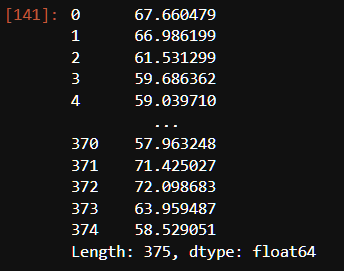
\includegraphics[scale = 0.65]{images/result_novomodel_11.png}
\label{filtro1}
\caption{Resultado de y\_pred com os novos dados - questão 11}
\end{figure}

Para o modelo de log(y), precisamos usar a expressão adequada para obter a previsão de y. Se os resíduos do modelo de log(y) forem normais, podemos simplesmente usar a exponencial da previsão do modelo para log(y). Caso contrário, precisamos aplicar uma correção nos valores previstos, como descrito nas notas de aula. Vamos verificar se os resíduos do modelo de log(y) são normais:


\begin{tcolorbox}[colback=white,boxrule=1pt,arc=5pt,auto outer arc]
  \begin{lstlisting}[language=Python]ed = 
import scipy.stats as stats
import matplotlib.pyplot as plt

residuos = model_outliers.resid

stats.probplot(residuos, dist='norm', plot=plt)
plt.show()

    \end{lstlisting}
\end{tcolorbox} \\

\begin{figure}[H]
\centering
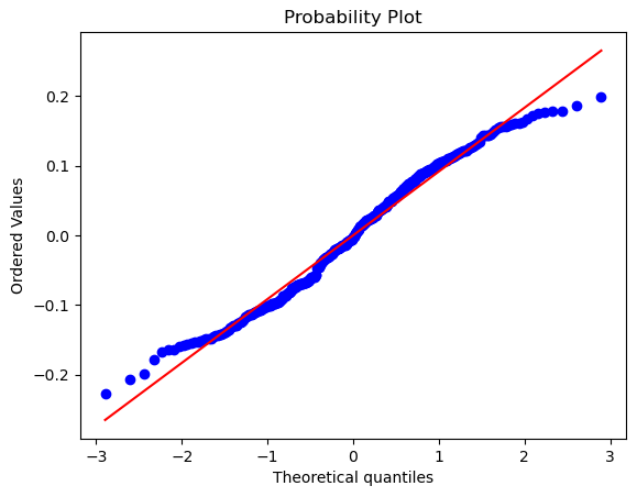
\includegraphics[scale = 0.65]{images/graph.png}
\label{filtro1}
\caption{Gráfico Q-Q plot}
\end{figure}

O gráfico Q-Q plot sugere que os resíduos do modelo de log(y) são aproximadamente normais. Portanto, podemos simplesmente usar a exponencial da previsão do modelo para log(y) para obter as previsões de y:\\

Para obter as previsões de y a partir do modelo para log(y), podemos utilizar a expressão:\\

$y = exp(\hat{y}_{log}) \cdot exp(\frac{1}{2}\hat{\sigma}^2)$

onde $\hat{y}_{log}$ é a previsão do modelo para log(y) e $\hat{\sigma}^2$ é a variância dos resíduos do modelo para log(y).\\

Podemos notar que que estamos multiplicando a previsão do modelo para log(y) pelo fator de correção $exp(\frac{1}{2}\hat{\sigma}^2)$ para levar em conta a transformação aplicada aos dados (logaritmo) e garantir que a previsão esteja na escala original (y).\\ \\

É importante lembrar que essa expressão só é válida se os resíduos do modelo para log(y) seguem uma distribuição normal. Caso contrário, outros métodos devem ser utilizados para obter as previsões de y.\\

No código abaixo, n\_model é o modelo ajustado com a transformação logarítmica, n\_X é a matriz de variáveis explicativas correspondente ao caso em questão, y\_pred\_log é a previsão de log(y) obtida pelo modelo para o caso em questão e y\_pred é a previsão correspondente de y. y\_pred\_list é uma lista que armazena as previsões de y para todos os casos.\\

\begin{tcolorbox}[colback=white,boxrule=1pt,arc=5pt,auto outer arc]
  \begin{lstlisting}[language=Python]ed = 

n_X = novo_df[['temp_med', 
                'temp_min', 
                'temp_max',
                'chuva_mm',
                'fds']]
n_y = novo_df['consumo']

# adicionando constante
n_X = sm.add_constant(n_X)

# ajustando o modelo de regressao
n_model = sm.OLS(n_y, n_X).fit()

y_pred = n_model.predict(n_X)

# Aplicando a exponencial para obter a previsao de y
y_pred_log = np.exp(y_pred)

# Calculando o MAPE para y_pred_log
mape_y = np.mean(
        np.abs((n_y - y_pred_log) / n_y)) * 100
        
# Calculando o MAPE para y_pred
mape_y_log = np.mean(np.abs((n_y - y_pred) / n_y)) * 100

print(str(mape_y ) + ", " + str(mape_y_log))

    \end{lstlisting}
\end{tcolorbox} \\


O MAPE para y\_pred\_log deu 84125591233553.03, enquanto que o MAPE para y\_pred deu 7.955114947975386.\\

Isso indica que o modelo obtido para y\_pred é mais preciso do que o modelo obtido para y\_pred\_log. O MAPE para y\_pred\_log é muito alto, o que indica que o modelo não está fazendo previsões precisas. Já o MAPE para y\_pred é bastante baixo, o que sugere que o modelo está se ajustando bem aos dados e é capaz de fazer previsões precisas.  Significa que as previsões do modelo, em média, apresentam um erro percentual absoluto de cerca de 7.96\%. Esse valor pode ser considerado razoável.




\newpage
% REFERENCIAS %%%%%%%%%%%%%%%%%%%%%%%%%%%%%%%%%%%%%%%%%%%%%%%%%%%%%%%%%%%%%%


\end{document}